%pir api
Pir API'en er implementeret i PSoC creator. Top designet består af en input pin (P1[1]) der modtager et signal fra pir-sensoren når der er bevægelse, se billedet \ref{lab:pir_topdesing}. Denne pin går ind og aktiverer en ISR routine. I source filen ses det at constructoren starter ISR routinen og destructoren stopper den. Selve ISR funktionen går ind og kalder en metode fra controlleren, der deaktivere sprinkleren og starter en timer på 30 min før der igen kan vandes.   

\begin{figure}[htb]
\centering
{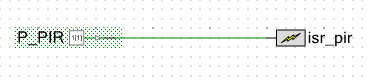
\includegraphics[width=0.60\textwidth]{filer/pics/pir_api_topdesign}}
\caption{Top Design for pir API}
\label{lab:pir_topdesing}
\end{figure}

\subsubsection*{Source fil}

\begin{lstlisting}[language=C]
//Constructor implementation
void pir_init()
{
    isr_pir_Start();
}

//Deconstructor implementaion
void pir_exit()
{
    isr_pir_Stop();
}

//ISR
extern void isr_pir_Interrupt()
{  
    loadData_movementDetekt();   
}
\end{lstlisting}